%-----------------------------------------------------------------
% LaTeX template for a document
% Written By: Pierre-Louis GAUTIER
% Date Updated: August 21, 2021 (v1.2.1)
%-----------------------------------------------------------------

\documentclass[a4paper, 11pt]{article}

% NOTE To conserve the space in the sentence passed as option to the package double braces to protect the spaces.
% It's an unfortunate feature of the core latex option handling

\usepackage[imageHeaderLeft     =   {clearWayShort.png},
            imageHeaderRight    =   {eseoShort.jpg},
            subject             =   {{}},
            keywords            =   {{}},
            encoding            =   {utf8},
            language            =   {french},
            showunnemberred     =   false
            ]{Parameter}

\usepackage[logoSchool  =   {eseoLong.jpg},
            logoCompany =   {clearWayLong.png},
            nameCompany =   {{ClearWay}},
            nameSchool  =   {{École d'Électronique de l'Ouest}},
            version     =   {0.1.0},
            statue      =   {{En cours}},
            texte       =   {{}}
            ]{FrontPage}

%%%%%%%%%%%%%%%%%%%%%%%%%%%%%%%%%%%%%%%%%%%%%%%%%%%%%%
%% Load the glossary from the given files %%

\newignoredglossary{ignored}

\makeglossaries
\loadglsentries{glossary.tex}
\loadglsentries[ignored]{glossary-ignored.tex}

%% Load the bibliography from the given files %%

\addbibresource{biblio.bib}

%% General config for header, footer and front page %%

\author{\glsentryname{leo}, \glsentryname{damien}, \glsentryname{pierreLouis}}
\title{Recherche}
\date{\normalsize\today} % Enter a custom date or let it, it's the current date

%%%%%%%%%%%%%%%%%%%%%%%%%%%%%%%%%%%%%%%%%%%%%%%%%%%%%%

\begin{document}

\maketitle

\newpage
\pagenumbering{arabic} % restart the page numbering
\thispagestyle{empty}

\begin{table}[ht]
    \centering
    \begin{xltabular}{\linewidth}{| c
        | >{\centering\arraybackslash}X
        | >{\centering\arraybackslash}p{2.1cm}
        | c|}

        \hline
        \rowcolor{tableColorDark}  Date & Action                                 & Auteur               & Version
        \endfirsthead
        \hline

        06 janvier 2022                 & Création du document                  & \gls{pierreLouis}    & v0.0.1  \\\hline
        06 janvier 2022                 & Rédaction du guide d'installation     & \gls{pierreLouis}    & v0.1.0  \\\hline
        07 janvier 2022                 & Rédaction du guide d'utilisation      & \gls{damien}         & v0.1.1  \\\hline
        07 janvier 2022                 & Ajout des arguments, options et toml  & \gls{damien}         & v0.1.2  \\\hline


    \end{xltabular}
    \label{tab:versionning}
\end{table}

\tableofcontents

\clearpage

\section{Comparaison des protocoles de communication}
\label{sec:comparaisonProtocoleCommnunication}

\subsection{Objectifs}
\label{sec:comparaisonProtocoleCommnunicationObjectifs}

L'objectif de cette étude est de comparer les différents protocoles et logiciels de communication
pouvant être utilisé dans ce projet afin de répondre au mieux aux différents besoins.\newline

Les différents critères étudiés sont :

\begin{itemize}
    \item Le mode de transmission et sa portée
    \item Le débit de la transmission
    \item La consommation énergétique
\end{itemize}

Les différents modes de communication et protocoles étudiés seront :

\begin{itemize}
    \item \nameref{sec:communicationRadio} :
          \begin{itemize}
              \item \Gls{wifi}
              \item \Gls{wimax}
              \item \Gls{bluetooth}
              \item \Gls{lorawan}
          \end{itemize}
    \item \nameref{sec:communicationFilaire} :
          \begin{itemize}
              \item \Gls{cpl}
              \item \Gls{ethernet}
          \end{itemize}
\end{itemize}

\subsection{Méthodologie de recherche}
\label{sec:centralise_Methodo}

La méthodologie de recherche sera orientée afin de trouver des résultats pertinents concernant :
\begin{itemize}
    \item Nos besoins par rapport aux cyclistes
    \item Les infrastructures déjà installés
    \item La longueur focale appropriée à notre besoin
    \item La distance, l'angle et la hauteur de la caméra par rapport à son environnement
\end{itemize}
Ces investigations seront menées grâce à internet en utilisant les filtres les plus pertinents pour chaque recherche.
Cela permettra d'avoir des résultats cohérents et de pallier les recherches personnalisées liées aux algorithmes de Google.
Pour ce qui est des spécifications de la caméra, nous étudierons ce qui se fait dans
le monde de la télésurveillance municipale en étudiant les spécifications des leaders du marché mondial.

\subsection{Résultats}
\label{sec:comparaisonProtocoleCommnunicationResultats}

\subsubsection{Les communications radio}
\label{sec:communicationRadio}

\paragraph{\glsentryname{wifi}}
\label{sec:wifi}

Il existe différentes versions et normes de \gls{wifi}, chacune ayant un débit et une portée différente.
La plupart des cartes réseaux sont adaptées pour la norme \textbf{802.11}, se divisant en différents standards
\cite{wifi}. Il est possible d’utiliser n’importe quel protocole de transport basé sur \gls{ip}.\newline

\begin{table}[H]
    \centering
    \rowcolors{2}{tableColor}{white}
    \begin{tabular}{|c|c|c|c|}
        % Header
        \hline
        \rowcolor{tableColorDark} Normes & Débit de données & Portées & Fréquence d'émission   \\
        \hline

        % Data
        \gls{wifi} 802.11a               & 30 Mbit/s        & 10 m    & 5 GHz                  \\\hline
        \gls{wifi} 802.11b               & 6 Mbit/s         & 300 m   & 2.4 GHz                \\\hline
        \gls{wifi} 802.11g               & 26 Mbit/s        & 70 m    & 2.4 GHz                \\\hline
        \gls{wifi} 802.11n               & 600 Mbit/s       & 70 m    & 2.4 GHz ou 5 GHz       \\\hline
        \gls{wifi} 802.11ac              & 7 Gbit/s         & 30 m    & 2.4 GHz et 5 GHz       \\\hline
        \gls{wifi} 802.11ax              & 10 Gbit/s        & 700 m   & Entre 2.4 GHz et 6 GHz \\\hline
    \end{tabular}
    \label{tab:debitPorteeWifi}
    \caption{Débit et portée du \glsentryname{wifi}}
    \nocite{debitPortee}
\end{table}

\paragraph{\glsentryname{wimax}}
\label{sec:wimax}

Le \gls{wimax} est un ensemble de normes techniques basées sur le standard de transmission radio \textbf{802.16}
permettant la transmission de données \gls{ip}.\newline
Il a pour principales particularités de supporter un haut débit de données (jusqu’à 75 Mbit/s en théorie, mais
excède rarement 20 Mbit/s sur quelques dizaines de kilomètres en condition réelle) sur des distances très importantes,
comprises entre 10 et 50 kilomètres selon les obstacles rencontrés par les ondes et de prioriser les usages de
la bande passante disponible entre les différents utilisateurs. \enquote{Ces qualités en font donc une sorte
    de \gls{wifi} survitaminé}{\cite{wimax}}.

\begin{table}[H]
    \centering
    \rowcolors{2}{tableColor}{white}
    \begin{tabular}{|c|c|c|c|}
        % Header
        \hline
        \rowcolor{tableColorDark} Normes & Débit de données & Portées & Fréquence d'émission   \\
        \hline

        % Data
        \gls{wimax} 802.16d              & 12 Mbit/s        & 20 km   & Entre 2 GHz et 11 GHz  \\\hline
        \gls{wimax} 802.16e              & 30 Mbit/s        & 3 km    & Entre 3.5 GHz et 6 GHz \\\hline
    \end{tabular}
    \label{tab:debitPorteeWimax}
    \caption{Débit et portée du \glsentryname{wimax}}
    \nocite{debitPortee}
\end{table}


\paragraph{\glsentryname{bluetooth}}
\label{sec:bluetooth}

Le \gls{bluetooth} sert à la transmission entre divers appareils numériques, avec ou sans connexion,
de données. Contrairement à d'autres technologies de transfert de données, il est
spécialisé dans les transferts sur des distances relativement courtes et une basse
consommation. Toutefois, il ne permet pas d'atteindre des débits de transfert élevés.\newline
Le \gls{bluetooth} se distingue du \gls{wifi} par une faible consommation énergétique. Il
ne nécessite en moyenne que 3\% de l'énergie nécessaire au \gls{wifi} pour la même tâche \cite{bluetoothConsumption}.
Le \gls{ble}, qui est une variante, permet une consommation encore plus faible.\newline
On peut résumer les performances du \gls{bluetooth} par ce tableau \cite{debitPortee, ble}.

\begin{table}[H]
    \centering
    \rowcolors{2}{tableColor}{white}
    \begin{tabular}{|c|c|c|c|}
        % Header
        \hline
        \rowcolor{tableColorDark} Normes & Débit de données & Portées & Fréquence d'émission \\
        \hline

        % Data
        \gls{bluetooth} 1.2              & 720 Kbit/s       & 10 m    & 2,4 GHz              \\\hline
        \gls{bluetooth} 2.0              & 2,1 Mbit/s       & 10 m    & 2,4 GHz              \\\hline
        \gls{bluetooth} 3.0              & 2,1 Mbit/s       & 10 m    & 2,4 GHz              \\\hline
        \gls{bluetooth} 4.x              & 3 Mbit/s         & 60 m    & 2,4 GHz              \\\hline
        \gls{bluetooth} 5.0              & 2 Mbit/s         & 200 m   & 2,4 GHz              \\\hline
        \gls{ble}                        & 1 Mbit/s         & 10 m    & 2,4 GHz ou 5 GHz     \\\hline
    \end{tabular}
    \label{tab:debitPorteeBluetooth}
    \caption{Débit et portée du \glsentryname{bluetooth}}
    \nocite{ble}\nocite{debitPortee}
\end{table}

\paragraph{\glsentryname{lorawan}}
\label{sec:lorawan}

Le protocole \gls{lorawan} se veut simple, peu coûteux à implémenter et économe en énergie plutôt que permettre des débits élevés en
utilisant la technologie \gls{lora} \cite{lorawan}. Cette technologie a pour priorité la faible consommation d'énergie.\newline

Tout comme le \gls{wimax}, le \gls{lorawan} a la capacité de prioriser les usages de la bande passante disponible en fonction
des besoins de chaque appareil et augmenter la durée de vie de la batterie.

\begin{table}[H]
    \centering
    \rowcolors{2}{tableColor}{white}
    \begin{tabular}{|c|c|c|c|}
        % Header
        \hline
        \rowcolor{tableColorDark} Normes & Débit de données         & Portées                        & Fréquence d'émission \\
        \hline

        % Data
        \gls{lora}                       & 10.3 kbit/s à 100 kbit/s & de quelques km à plus de 10 km & 868 MHz en Europe    \\\hline
    \end{tabular}
    \label{tab:debitPorteeLora}
    \caption{Débit et portée du \glsentryname{lora}}
    \nocite{debitPortee}
\end{table}

\subsubsection{Les communications filaires}
\label{sec:communicationFilaire}

\paragraph{\glsentryname{cpl}}
\label{sec:cpl}

\blockquote{Le principe des \gls{cpl} consiste à superposer au courant électrique alternatif de 50 ou 60 Hz
    un signal à plus haute fréquence et de faible énergie. Ce deuxième signal se propage sur l’installation
    électrique et peut être reçu et décodé à distance. Ainsi le signal \gls{cpl} est reçu par tout récepteur
    \gls{cpl} de même catégorie se trouvant sur le même réseau électrique. Cette façon de faire comporte cependant un
    inconvénient : le réseau électrique n'est pas adapté au transport de hautes fréquences, car il n'est pas blindé.
    En conséquence, la plus grande partie de l'énergie injectée par le modem \gls{cpl} est rayonnée sous forme
    d'onde radio.}{\cite{cpl}}

La technologie \gls{cpl} permet donc de mettre en place un réseau de communication par-dessus un réseau électrique sans
avoir à mettre en place plus d'infrastructures. Le \gls{cpl} est déjà utilisé dans l'industrie, notamment par \textit{Enedis}
avec les compteurs \textit{Linky}. Les débits atteints sont compris entre 14 et 1 200 Mbit/s.

\begin{table}[H]
    \centering
    \rowcolors{2}{tableColor}{white}
    \begin{tabular}{|c|c|}
        % Header
        \hline
        \rowcolor{tableColorDark} Normes & Débit de données         \\
        \hline

        % Data
        \gls{cpl}                        & 14 Mbit/s à 1 200 Mbit/s \\\hline
    \end{tabular}
    \label{tab:debitCPL}
    \caption{Débit du \glsentryname{cpl}}
    \nocite{cpl}
\end{table}

\paragraph{\glsentryname{ethernet}}
\label{sec:ethernet}

\Gls{ethernet} est le réseau le plus commun, les cartes réseaux les plus courantes le supportent. C'est une technologie
orientée pour des réseaux locaux, généralement dans un même bâtiment. Il existe différents standards avec des débits et des
types de câbles différents \cite{debitEthernet}.

\begin{table}[H]
    \centering
    \rowcolors{2}{tableColor}{white}
    \begin{tabular}{|c|c|c|c|}
        % Header
        \hline
        \rowcolor{tableColorDark} Standard \glsentryname{ethernet} & Débit de données & Câble                                & Distance maximale \\
        \hline

        % Data
        10Base2                                                    & 10 Mbit/s        & Câble coaxial de faible diamètre     & 185 m             \\\hline
        10Base5                                                    & 10 Mbit/s        & Câble coaxial de gros diamètre       & 500 m             \\\hline
        10Base-T                                                   & 10 Mbit/s        & Paire torsadée (catégorie 3)         & 100 m             \\\hline
        100Base-TX                                                 & 100 Mbit/s       & Double paire torsadée (catégorie 5)  & 100 m             \\\hline
        100Base-FX                                                 & 100 Mbit/s       & Fibre optique multimode              & 2 km              \\\hline
        1000Base-T                                                 & 1000 Mbit/s      & Double paire torsadée (catégorie 5e) & 100 m             \\\hline
        1000Base-LX                                                & 1000 Mbit/s      & Fibre optique monomode / multimode   & 500 m - 1 km      \\\hline
        1000Base-SX                                                & 1000 Mbit/s      & Fibre optique multimode              & 500 m             \\\hline
        10GBase-SR                                                 & 10 Gbit/s        & Fibre optique multimode              & 500 m             \\\hline
        10GBase-LX4                                                & 10 Gbit/s        & Fibre optique multimode              & 500 m             \\\hline
    \end{tabular}
    \label{tab:debitEthernet}
    \caption{Débit de l'\glsentryname{ethernet}}
    \nocite{debitEthernet}
\end{table}

\subsection{Conclusion}
\label{sec:comparaisonProtocoleCommnunicationConclusion}

Cette recherche sur les différents moyens de transmettre les informations au sein de \gls{sae} avait pour ambition de trouver le meilleur compromis entre
la consommation énergétique, le débit et la portée.
Il a fallu dans un premier temps réunir les informations, les analyser et les traiter afin de pouvoir les exploiter.\newline

En fonction de la manière dont \gls{sae} sera conçu, c'est-à-dire de manière décentralisée ou centralisée (voir partie \ref{sec:centralise}), alors les
besoins ne seront pas les mêmes.
Il faut toutefois noter la nécessité de faire un choix entre un mode de transmission radio ou filaire.\newline

Dans le cas d'une transmission radio, le \gls{wimax} semble être la technologie la plus adaptée pour un système centralisé.
En effet, le \gls{wifi} et le \gls{bluetooth} ont une portée insuffisante, tandis que le \gls{lora} possède un débit trop faible,
ne répondant pas à nos besoins. Toutefois, dans un contexte décentralisé, le \gls{wifi} semble être lui le plus adapté.\newline

Du côté des transmissions filaires, le \gls{cpl} semble le plus adapté, en effet le débit peut être suffisant et sa porté quasiment illimitée, malgré
d'importante perte énergétique. \Gls{ethernet} est plus adapté dans un contexte décentralisé, avec un débit important et une perte énergétique
plus faible que le \gls{cpl}.

\clearpage
%auteur : Damien Frissant

\section{Analyse pour la caméra}
\label{sec:camera}

\subsection{Objectifs}
\label{sec:camera_Objectifs}

Notre système \gls{sae} sera équipé d'une caméra permettant de détecter les cyclistes.
Il est important de trouver le meilleur positionnement et la meilleure configuration
de cette dernière par rapport à son environnement afin d'optimiser la détection des cyclistes.

De ce fait, nous chercherons les paramètres optimaux permettant de pallier la problématique de notre sujet.

\subsection{Méthodologie de recherche}
\label{sec:camera_Methodo}

La méthodologie de recherche sera orientée afin de trouver des résultats pertinents concernant :
\begin{itemize}
    \item Nos besoins par rapport aux cyclistes
    \item Les infrastructures déjà installés
    \item La longueur focale appropriée à notre besoin
    \item La distance, l'angle et la hauteur de la caméra par rapport à son environnement
\end{itemize}
Ces investigations seront menées grâce à internet en utilisant les filtres les plus pertinents pour chaque recherche.
Cela permettra d'avoir des résultats cohérents et de pallier les recherches personnalisées liées aux algorithmes de Google.
Pour ce qui est des spécifications de la caméra, nous étudierons ce qui se fait dans
le monde de télésurveillance municipale en étudiant les spécifications des leaders du marché mondial.

\subsection{Résultats}
\label{sec:camera_resultats}

\subsubsection{Nos besoins par rapport aux cyclistes}
\label{sec:camera_cycliste}

Pour dimensionner au mieux les paramètres de la caméra, il faut déjà savoir quelle peut être la vitesse maximale d’un cycliste.
Nous considérons que notre système sera installé majoritairement en ville.
En prenant en compte un cycliste circulant entre 10 km/h (2,8 m/s) et 50 km/h (14 m/s) nous réunissons la majorité des usagers.
En prenant le cas le plus extrême, 50 km/h, il nous faudrait soit :
\begin{itemize}
    \item Une distance de détection inférieure à 14 mètres, nécessitant minimum deux images par seconde.
    \item Une distance de détection comprise entre 14 et 19 mètres et une acquisition de deux images par seconde afin
          d’être sûr de voir l’usager.
    \item Une distance de détection comprise entre 20 et 30 mètres et une acquisition d’image d'une image par seconde qui permet
          de ménager les ressources de calcul de l’algorithme.
    \item Une distance de détection à plus de 30 mètres et une acquisition de moins d'une image par seconde.
\end{itemize}
D'un point de vue matériel, il parait plus évident de soulager les calculs en ayant moins de traitement à faire.

Ainsi, nous éliminons les cas où la distance de détection est trop faible, car le nombre d'images par seconde est conséquent.
Dans le cas, il faudra beaucoup de ressources logicielles et énergétiques pour que \gls{sae} fonctionne.
De plus, il n'est pas optimal d'avoir une distance de détection trop élevée.
En effet, si la distance de détection est trop large, notre système ne fonctionnera pas correctement.
Prenons l'exemple d'un système où notre panneau et la caméra se trouvent au même endroit et que l'algorithme de détection est idéal,
c'est-à-dire qu'il analyse en temps réel l'image reçue.
\begin{example}
    Si un cycliste est détecté à 80 mètres et qu'il roule à 10 km/h, il faudrait 30 secondes pour qu'il arrive à l'intersection,
    tandis que s'il roule à 50 km/h il lui faut que cinq secondes. La plage temporaire est trop large,
    car on ne peut pas allumer le panneau pendant 30 secondes, car c'est trop long. Il faudrait pouvoir détecter la vitesse des usagers.
    De plus, dans le cas où le cycliste circule à grande vitesse, le temps d'affichage du panneau est trop court.
\end{example}


Idéalement, il faudrait orienter la caméra afin d'avoir une période se rapprochant d'une image par seconde, tout en ayant une détection optimale.
Ainsi nous allons nous intéresser aux cas où le champ de vision de la caméra est compris entre 14 et 30 mètres.

\subsubsection{Infrastructures déjà installées dans les villes}
\label{sec:camera_infra}
Les caméras de surveillance sont de plus en plus présentes dans nos villes. Ces dispositifs peuvent être utiles à notre projet en cas d'évolution.
En effet, si nous réfléchissons \gls{sae} de façon à ce que le système de caméra se rapproche de celui des infrastructures déjà en place,
il sera plus aisé de faire évoluer le système de façon à ce qu'il s'intègre à ces dispositifs.
Il n'y a aucun standard concernant l'installation d'une caméra de surveillance. Néanmoins, nous pouvons exclure celles qui sont rotatives.
Pour celles qui sont fixes, elles sont installées entre 2m40 et 3m20. Les caractéristiques de ces dernières sont détaillés dans les paragraphes qui suivent.

\subsubsection{Longueur focale appropriée à notre besoin}
\label{sec:camera_focale}

\blockquote{La longueur focale nous indique le champ angulaire (la partie de la scène qui sera capturée)
    et le grossissement (la taille des éléments individuels).
    Plus la longueur focale est étendue, plus le champ angulaire est étroit et plus le grossissement est élevé.
    Plus la longueur focale est courte, plus l’angle de vue est large et plus le grossissement est réduit.}{\cite{focale}}

En plus de la focale, le champ de vision d'une caméra peut évoluer entre deux caméras ayant la même longueur focale
si elles ont une taille de capteur différent.
En effet, une caméra ou un appareil photo est vendu avec un \gls{CROP} qui est propre à chaque taille de capteur.
Ce désagrément peut être compensé par une longueur focale plus faible.
Le capteur plein format est la référence afin d'énoncer la longueur focale.
Pour nous rendre compte des écarts qu'il y a entre la taille d'une image en plein format et ce qui est vraiment perçu par l'appareil,
les longueurs focales qui suivent seront converties en équivalent plein format lorsqu'il y aura la mention \gls{epf}.

Comme indiqué ci-dessus, nous recherchons une solution permettant d'avoir une distance de détection importante.
Pour ce faire, il faut avoir une distance focale faible, inférieur à 25 mm (\gls{epf}).

En parcourant le site des leaders mondiaux de caméras de surveillance extérieures fixes
(Pelco \cite{pelco}, Axis \cite{axis} et Panasonic \cite{panasonic})
nous arrivons au constat qu'une focale pour les caméras de surveillance fixes est comprise entre 2,8 mm et 8,3 mm, mais que toutes ces caméras ont des capteurs compacts, donc ayant un coefficient multiplicateur élevé.
En effet, si on prend l'exemple des produits ci-dessus, la taille du capteur est comprise entre 1/3"(3,6 x 4,8 mm) et 1"(13,2 x 8,8 mm).
Pour connaitre l'équivalent en termes de distance focale, il faut faire le rapport entre la taille d'un capteur plein format (36 x 24 mm)
et celui du capteur de la caméra pour laquelle on veut le coefficient multiplicateur :
\begin{itemize}
    \item Pour le modèle Axis Q1645 \cite{axisQ1645}, on a une taille de capteur de 1/2"
          ce qui fait un coefficient multiplicateur de 5,625x. C'est-à-dire que malgré une distance focale annoncée de 3.9 mm, son \gls{epf} est de 22 mm.
    \item Pour le modèle Panasonic i-Pro Extreme WV-S1531LN \cite{panaIPro}.
          la taille du capteur est de 1/3", ce qui fait un coefficient multiplicateur de 10x. Ainsi, même si la distance focale minimale est annoncée à 2,8 mm, son \gls{epf} est de 28 mm.
\end{itemize}

Nous pouvons également avoir une distance de détection importante en ayant une focale plus longue. Pour ce faire il faut une inclinaison moindre entre cette dernière et le sol.


\subsubsection{La distance, angle et hauteur de la caméra}
\label{sec:camera_distance}
D'après les résultats précédents, nous avons accès nos recherches sur des caméras ayant une focale faible.

La hauteur idéale du système serait celle se rapproche le plus possible de celle d'une personne sur un vélo (comprise en un mètre et deux mètres).
L'inconvénient d'un tel dispositif, c'est l'obstruction du champ de vision par un élément tiers, une voiture, un camion, etc. Pour pallier ce problème,
la caméra devra se trouver à une hauteur supérieure de deux mètres, sans pour autant être trop haute. En effet, plus l'appareil est haut,
plus le champ de vision est grand et ce n'est pas ce que l'on recherche.

En étudiant les manuels d'installation des fabricants de caméras \cite{ganz}, nous obtenons les paramètres suivants :

\begin{table}[ht!]
    \centering
    \begin{tabular}{|l|l|l|l|l|}
        \hline
        \rowcolor{tableColor}
        \cellcolor{tableColor}                           & Focale  & 3,3mm   & \cellcolor{tableColor}                           & \cellcolor{tableColor}                                            \\ \cline{2-3}
        \rowcolor{tableColor}
        \cellcolor{tableColor}                           & Hauteur & 2,70m   & \cellcolor{tableColor}                           & \cellcolor{tableColor}                                            \\ \cline{2-3}
        \rowcolor{tableColor}
        \multirow{-3}{*}{\cellcolor{tableColor}Config 1} & Angle   & 85°     & \multirow{-3}{*}{\cellcolor{tableColor}Résultat} & \multirow{-3}{*}{\cellcolor{tableColor}\begin{tabular}[c]{@{}l@{}}Ces paramètres correspondent à la distance maximale \\ de reconnaissance. Une voiture peut être détectée à 80 \\ mètres grâce à cette configuration\end{tabular}} \\ \hline
                                                         & Focale  & 4 mm    &                                                  &                                                                   \\ \cline{2-3}
                                                         & Hauteur & 3 m     &                                                  &                                                                   \\ \cline{2-3}
        \multirow{-3}{*}{Config 2}                       & Angle   & 70°     & \multirow{-3}{*}{Résultat}                       & \multirow{-3}{*}{\begin{tabular}[c]{@{}l@{}}La caméra est capable de détecter un objet à plus de \\ 20 mètres. \\ Dans ce cas, 99\% des objets à détecter le sont.\end{tabular}}                       \\ \hline
        \rowcolor{tableColor}
        \cellcolor{tableColor}                           & Focale  & 4 mm    & \cellcolor{tableColor}                           & \cellcolor{tableColor}                                            \\ \cline{2-3}
        \rowcolor{tableColor}
        \cellcolor{tableColor}                           & Hauteur & 3 m     & \cellcolor{tableColor}                           & \cellcolor{tableColor}                                            \\ \cline{2-3}
        \rowcolor{tableColor}
        \multirow{-3}{*}{\cellcolor{tableColor}Config 3} & Angle   & 10°     & \multirow{-3}{*}{\cellcolor{tableColor}Résultat} & \multirow{-3}{*}{\cellcolor{tableColor}\begin{tabular}[c]{@{}l@{}}La distance et l’angle ne sont pas optimaux. \\ En effet, peu de symbole sont reconnus dans une \\ image ayant cette configuration.\end{tabular}} \\ \hline
                                                         & Focale  & 4 mm    &                                                  &                                                                   \\ \cline{2-3}
                                                         & Hauteur & 25-31 m &                                                  &                                                                   \\ \cline{2-3}
        \multirow{-3}{*}{Config 4}                       & Angle   & 60°     & \multirow{-3}{*}{Résultat}                       & \multirow{-3}{*}{\begin{tabular}[c]{@{}l@{}}Ces paramètres offres un champ de vision de plus de \\ 30 mètres, près de 99\% des symboles sont reconnus. \\ Néanmoins, la détection dépend beaucoup de l'angle \\ des symboles arrivant.\end{tabular}}                       \\ \hline
        \rowcolor{tableColor}
        \cellcolor{tableColor}                           & Focale  & 4 mm    & \cellcolor{tableColor}                           & \cellcolor{tableColor}                                            \\ \cline{2-3}
        \rowcolor{tableColor}
        \cellcolor{tableColor}                           & Hauteur & 10-16 m & \cellcolor{tableColor}                           & \cellcolor{tableColor}                                            \\ \cline{2-3}
        \rowcolor{tableColor}
        \multirow{-3}{*}{\cellcolor{tableColor}Config 5} & Angle   & 10°     & \multirow{-3}{*}{\cellcolor{tableColor}Résultat} & \multirow{-3}{*}{\cellcolor{tableColor}\begin{tabular}[c]{@{}l@{}}À l’instar de la configuration 3, le taux de \\ reconnaissance est nettement dégradé avec \\ un angle si faible.\end{tabular}} \\ \hline
                                                         & Focale  & 2.4 mm  &                                                  &                                                                   \\ \cline{2-3}
                                                         & Hauteur & 2 m     &                                                  &                                                                   \\ \cline{2-3}
        \multirow{-3}{*}{Config 6}                       & Angle   & 90°     & \multirow{-3}{*}{Résultat}                       & \multirow{-3}{*}{\begin{tabular}[c]{@{}l@{}}Détection rapide et fiable des usagers de la route. \\ Néanmoins, si un cycliste se trouve derrière \\ un SUV, il ne sera pas détecté.\end{tabular}}                      \\ \hline
    \end{tabular}
    \caption{Comparatif des différentes configurations d'une caméra}
    \label{fig:comparatifCamera}
\end{table}

Nous pouvons observer que toutes les caméras ayant un angle compris entre 0-10° et 80-90° ne conviennent pas à nos attentes.
Soit le champ de vison est trop large soit trop étroit. Ainsi, elles ne seront pas adaptées à notre besoin.
Les appareils se trouvant à une distance supérieure de 10 mètres ne correspondent pas aux dispositifs fixes de surveillance présents dans les villes aujourd'hui.

Cela nous permet d'éliminer cinq configurations, ainsi ils nous restent uniquement la deuxième configuration,
qui correspond aux exigences spécifiées dans le paragraphe \ref{sec:camera_cycliste}.


\subsection{Conclusion}
\label{Conclusion}
Cette recherche concernant les caméras avait pour ambition de trouver le meilleur compromis afin de détecter un cycliste.
Il a fallu dans un premier temps réunir les informations, les analyser, les traiter et établir une conclusion pour chaque sous-partie.

En prenant en compte la vitesse maximale d'un cycliste, nous sommes arrivés à quatre dispositifs possibles. Nous avons constaté qu'il était intéressant
d'avoir une détection nécessitant peu d'image par seconde. En effet, cela permet d'avoir un système moins gourmand en ressources logicielles.

Les paramètres permettant de régler physiquement une caméra de détection sont primordiaux afin que le système soit optimisé.
En effet, si la caméra est mal orientée il faudra traiter trop de donnée dans un cas, ce qui est énergivore ou pas assez donnée, ce qui est inefficace.
Voyons ce que nos recherches nous ont enseignées :

\subsubsection*{Distance focale}
En nous renseignant sur les différentes caméras fixes de vidéo-surveillance installées, il s’avère que les caméras utilisées embarquent un grand angle.
Pour notre système, il est également important de choisir une longueur focale proche de celles présentes sur les infrastructures déjà existantes.
En effet, ça permettra d'avoir un système plus évolutif, si nous voulons implémenter \gls{sae} sur le matériel déjà présent dans les villes.
D'après la section \ref{sec:camera_focale}, il faudrait que la focale soit comprise entre 1.8 mm et 3.8 mm pour se rapprocher au plus de ces dispositifs.
De plus, quel que soit le coefficient multiplicateur, un tel optique aura une focale (\gls{epf}) acceptable.

\subsubsection*{Hauteur}

Comme décrit dans le paragraphe \ref{sec:camera_distance}, il faut que l'objectif surpasse les voitures afin de pouvoir voir derrière elles.
Dans le cas contraire, \gls{sae} pourrait ne pas voir des cyclistes alors qu'ils se trouvent derrière des voitures.
Ainsi une haute comprise entre 2m50 et 3m60 semble convenir à nos besoins, de plus c'est la hauteur à laquelle se trouve la vidéosurveillance des villes.

\subsubsection*{Angle de vue}
Nous avons pu voir que l'angle de vue de la caméra influence la détection des symboles dans l'image. Une détection correcte se trouve entre 90° et 60°.
Néanmoins, d'après les conclusions précédentes, nous considérerons que l'angle optimal est de 70°.

\subsubsection*{Distance de détection}
Nous avons vu qu'un champ de vision trop grand n'aide pas à servir notre problème. Dans le cas contraire la distance est trop faible pour analyser correctement l'image.
Les résultats des parties \ref{sec:camera_cycliste} et \ref{sec:camera_distance} sont très proches.
La première section mentionne une distance de détection de 14 à 30 mètres. Pour la seconde, la distance de détection est de 20 mètres.
Cette distance est suffisante afin d'avoir qu'une image par seconde à traiter. Néanmoins, il ne s'agit pas de jouer avec la sécurité des cyclistes.
Si le matériel le permet, il est conseillé de doubler le nombre d'images par seconde.


\clearpage
%auteur : Damien Frissant

\section{Serveur centralisé versus serveur décentralisé}
\label{sec:centralise}

\subsection{Objectifs}
\label{sec:centralise_Objectifs}
Le but de cette section est de déterminer quelle organisation est mieux adaptés au projet ClearWay entre un dispositif centralisé ou décentralisé.

\subsection{Méthodologie de recherche}
\label{sec:centralise_Methodo}
Se référer à la partie \ref{sec:camera_Methodo}.

\subsection{Résultats}
\label{sec:centralise_Resultats}

\subsubsection{Serveur centralisé}
\label{sec:centralise_centralise}
Un système centralisé est composé d'une machine qui centralise et traite toutes les informations.

\enquote{
    Ils sont aussi plus faciles à mettre au point, et à déboguer – quand une erreur arrive, on n’a pas à se demander d’où elle provient. \cite{centraliser}
}
Un serveur centralisé à l'avantage de ne pas avoir besoin d'implémenter cette technologie à chaque intersection que l'on souhaite protéger avec ClearWay.
Néanmoins, ces systèmes sont critiques et fragile, car un dysfonctionnement a des conséquences sur tous les dispositifs actifs.
La capacité d'un serveur est limité, s'il y a beaucoup de données à traiter il y a des risques de saturation.
De plus il faut une communication ayant un débit correct et une portée suffisante. Cela implique d'éventuelles infrastructures (se référer à la partie \ref{sec:comparaisonProtocoleCommnunication}).
Un serveur centralisé permettrait d'implémenter notre solution au sein d'un poste de commandement sécurité d'une ville. De ce fait,
le dispositif serait moins coûteux à installer pour les collectivités et profiterait à plus de personnes.

\subsubsection{Serveur décentralisé}
\label{sec:centralise_decentralise}
Un système décentralisé peut être vu comme une fourmilière. Par exemple internet est un système décentralisé, où il n'y a des millions de machines autonomes. Il n'y a pas de machine centrale.
Il est facile à mettre en place à des endroits qui ne sont pas relié à un poste de sécurité.
En opposition aux serveurs centralisés, ceux qui sont décentralisés ont une résistance aux attaques, car tous les serveurs sont indépendants.

\subsubsection{Résultats}
\label{sec:centralise_resultat}
En conclusion, il n'y a pas de bon choix entre un système centralisé et décentralisé.
Dans un premier temps, nous allons créer un système décentralisé afin de contrôler le système entièrement. En effet, il est intéressant
d'avoir un prototype fonctionnel dans son ensemble, où l'on peut nous même contrôler la caméra.

Une fois le prototype décentralisé opérationnel, nous pourrons étudier la version centraliser permettant d'équiper des carrefours ayant des caméras à proximité.

\clearpage
\section{Comparaison des bibliothèques d'intelligence artificielle}
\label{sec:comparaisonIA}

\subsection{Objectifs}
\label{sec:comparaisonIA:objectifs}

L'objectif de cette étude est de comparer plusieurs bibliothèques d'intelligence artificielle
permettant de détecter des cyclistes à partir d'une vidéo.

\subsection{Méthode de recherche}
\label{sec:comparaisonIA:methode_recherche}

Après quelques recherches, nous avons trouvé 2 bibliothèques d'intelligence artificielle
qui permettent de détecter des objets à partir d'une vidéo : ImageAI et OpenCV.
Elles fonctionnent avec le langage de programmation Python.

\subsubsection{ImageAI}
\label{sec:comparaisonIA:methode_recherche:imageAI}

ImageAI dispose de fonctions déjà prêtes pour réaliser de la détection d'objets dans une vidéo.
Avec cette bibliothèque, cette détection est possible avec un code d'une dizaine de lignes.
Elle offre le choix de la vitesse de détection : normal, fast, faster, fastest et flash.

\subsubsection{OpenCV}
\label{sec:comparaisonIA:methode_recherche:openCV}

OpenCV laisse au codeur le soin de récupérer la position des objets, leur probabilité, et de dessiner un cadre autour de ces objets.
Avec cette bibliothèque, une cinquantaine de lignes de code est nécessaire.
Elle propose d'utiliser un algorithme étant entraîné à différentes tailles d'images : (320px, 320px), (416px, 416px) ou (608px, 608px).

\subsubsection{Règles à suivre par les programmes}
\label{sec:comparaisonIA:methode_recherche:regles}
Dans un premier temps, nous avons testé des programmes utilisant les bibliothèques ImageAI et OpenCV \cite{ImageAI, OpenCV}.
Puis, nous avons adapté ces programmes à nos besoins.
Afin de pouvoir comparer ces 2 bibliothèques, nous avons fixé les règles que nos 2 programmes doivent suivre :

\begin{itemize}
    \item Détecter seulement les cyclistes et ignorer les autres objets
    \item Considérer que les cyclistes sont détectés lorsqu'ils le sont avec une probabilité de minimum 50\%
    \item Lorsqu'un cycliste est détecté, afficher un message dans la console avec la probabilité associée
    \item Réaliser un fichier vidéo de sortie au format "avi" ayant une image par seconde, et contenant des cadres autour des cyclistes détectés avec leur probabilité associée
    \item Utiliser l'algorithme d'intelligence artificielle YOLOv3
\end{itemize}

\subsubsection{L'algorithme YOLO}
\label{sec:comparaisonIA:methode_recherche:yolo}

YOLO est l'acronyme de "You Only Look Once". Cela traduit le fait qu'un seul réseau de neurone est utilisé. \cite{Yolov3}
Ce dernier divise les images d'une vidéo en régions, et prédit des cadres contenant des objets avec leur probabilité pour chaque région.
Ensuite, seuls les cadres contenant des objets avec une probabilité assez forte sont conservés.
Nous utilisons la version 3 de YOLO qui date de 2018, car celle-ci est à la fois supportée par ImageAI et OpenCV.

\subsubsection{Méthode de comparaison}
\label{sec:comparaisonIA:methode_recherche:methode_comparaison}

Nous avons comparé nos 2 programmes utilisant respectivement les bibliothèques ImageAI et OpenCV avec leurs différents paramètres.
Le programme utilisant ImageAI a donc été testé avec ses différentes vitesses de détection : normal, fast, fastest et flash.
La vitesse "faster" a été écartée car elle ne permettait pas de détecter de vélo sur notre vidéo de référence.
De même, le programme utilisant OpenCV a été testé avec un algorithme étant entraîné à différentes tailles d'images :
(320px, 320px), (416px, 416px) et (608px, 608px).

La \gls{video de reference} que nous avons utilisée est une vidéo de 15 secondes suivant un cycliste sur une route.
Lorsque nous effections des tests avec la vidéo originale ayant 30 images par seconde (ips),
le temps de traitement de cette vidéo dépassait les 3 minutes.
Nous avons donc choisi de tester cette vidéo avec 1 ips, 2 ips et 3 ips.

Pour comparer nos 2 programmes avec leurs différents paramètres, nous avons réalisé un programme en Python permettant
d'exécuter ces programmes tout en calculant leur temps d'exécution.
Cela affiche ensuite ces différents temps sous la forme d'un diagramme en bâtons grâce à la bibliothèque matplotlib.
Nous avons également réalisé un tableau montrant l'efficacité des 2 programmes suivant leurs différents paramètres.

Ces tests ont été réalisé à partir d'un ordinateur ayant les paramètres suivant :
\begin{itemize}
    \item Type : VivoBook\_ASUSLaptop X521FA\_K533FA 1.0
    \item Système d'exploitation utilisé : Linux
    \item Distribution utilisée : Ubuntu 20.04.3 LTS x86\_64
    \item \gls{CPU} : Intel i7-10510U (8) @ 4.900GHz
    \item \gls{GPU} : Intel CometLake-U GT2 [UHD Graphics]
\end{itemize}
Il est à noter que cet ordinateur ne dispose pas de GPU NVIDIA, ce qui aurait augmenté la rapidité des tests.

\subsection{Résultats}
\label{sec:comparaisonIA:resultats}

\subsubsection{Comparaison à 1 image par seconde}
\label{sec:comparaisonIA:resultats:1fps}

\begin{figure}[H]
    \centering
    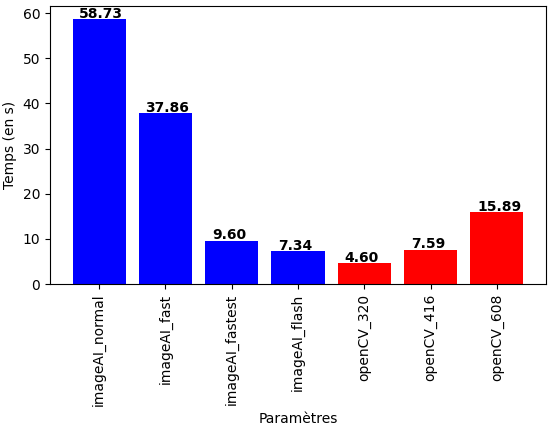
\includegraphics[width=0.7\textwidth]{img/result_1fps.png}
    \caption{Comparaison des bibliothèques ImageAI et OpenCV à 1 ips}
\end{figure}

Le tableau~\ref{tab_1fps} présente l'efficacité des 2 programmes suivant leurs différents paramètres à 1 ips.
Il renseigne le nombre de fois que le vélo a été détecté sur la vidéo ayant 1 ips.
Lorsque le vélo est détecté 2 fois sur une image, cela n'est pas pris en compte dans le nombre de détections.
Cependant, cela apparaît dans la colonne "Détection en double".

\begin{table}[H]
    \centering
    \rowcolors{2}{tableColor}{white}
    \begin{tabular}{|c|c|c|c|}
        \hline
        \rowcolor{tableColorDark} Paramètres & Nb de détections & Détection en double \\
        \hline

        imageAI\_normal                      & 9                & 1                   \\\hline
        imageAI\_fast                        & 8                & 0                   \\\hline
        imageAI\_fastest                     & 6                & 0                   \\\hline
        imageAI\_flash                       & 5                & 0                   \\\hline
        openCV\_320                          & 9                & 0                   \\\hline
        openCV\_416                          & 9                & 0                   \\\hline
        openCV\_608                          & 8                & 1                   \\\hline
    \end{tabular}
    \caption{Comparaison de l'efficacité des 2 programmes suivant leurs différents paramètres à 1 ips}
    \label{tab_1fps}
\end{table}

\subsubsection{Comparaison à 2 images par seconde}
\label{sec:comparaisonIA:resultats:2fps}

\begin{figure}[H]
    \centering
    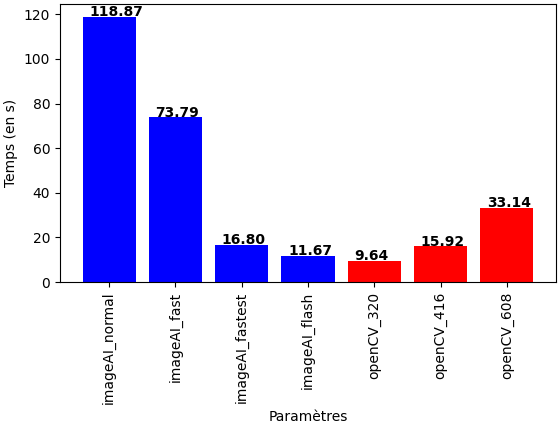
\includegraphics[width=0.7\textwidth]{img/result_2fps.png}
    \caption{Comparaison des bibliothèques ImageAI et OpenCV à 2 ips}
\end{figure}

Le tableau~\ref{tab_2fps} présente l'efficacité des 2 programmes suivant leurs différents paramètres à 2 ips.
Il renseigne le nombre de fois que le vélo a été détecté sur la vidéo ayant 2 ips.
Lorsque le vélo est détecté 2 fois sur une image, cela n'est pas pris en compte dans le nombre de détections.
Cependant, cela apparaît dans la colonne "Détection en double".

\begin{table}[H]
    \centering
    \rowcolors{2}{tableColor}{white}
    \begin{tabular}{|c|c|c|c|}
        \hline
        \rowcolor{tableColorDark} Paramètres & Nb de détections & Détection en double \\
        \hline

        imageAI\_normal                      & 14               & 1                   \\\hline
        imageAI\_fast                        & 14               & 0                   \\\hline
        imageAI\_fastest                     & 11               & 0                   \\\hline
        imageAI\_flash                       & 9                & 0                   \\\hline
        openCV\_320                          & 15               & 0                   \\\hline
        openCV\_416                          & 16               & 0                   \\\hline
        openCV\_608                          & 14               & 0                   \\\hline
    \end{tabular}
    \caption{Comparaison de l'efficacité des 2 programmes suivant leurs différents paramètres à 2 ips}
    \label{tab_2fps}
\end{table}

\subsubsection{Comparaison à 3 images par seconde}
\label{sec:comparaisonIA:resultats:3fps}

\begin{figure}[H]
    \centering
    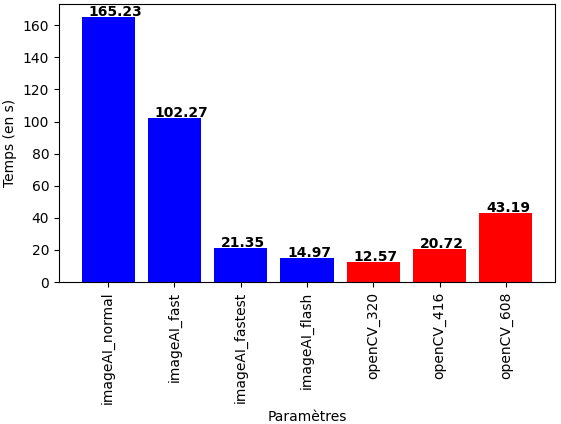
\includegraphics[width=0.7\textwidth]{img/result_3fps.png}
    \caption{Comparaison des bibliothèques ImageAI et OpenCV à 3 ips}
\end{figure}

Le tableau~\ref{tab_3fps} présente l'efficacité des 2 programmes suivant leurs différents paramètres à 3 ips.
Il renseigne le nombre de fois que le vélo a été détecté sur la vidéo ayant 3 ips.
Lorsque le vélo est détecté 2 fois sur une image, cela n'est pas pris en compte dans le nombre de détections.
Cependant, cela apparaît dans la colonne "Détection en double".

\begin{table}[H]
    \centering
    \rowcolors{2}{tableColor}{white}
    \begin{tabular}{|c|c|c|c|}
        \hline
        \rowcolor{tableColorDark} Paramètres & Nb de détections & Détection en double \\
        \hline

        imageAI\_normal                      & 20               & 1                   \\\hline
        imageAI\_fast                        & 20               & 0                   \\\hline
        imageAI\_fastest                     & 16               & 0                   \\\hline
        imageAI\_flash                       & 13               & 0                   \\\hline
        openCV\_320                          & 21               & 0                   \\\hline
        openCV\_416                          & 22               & 0                   \\\hline
        openCV\_608                          & 22               & 0                   \\\hline
    \end{tabular}
    \caption{Comparaison de l'efficacité des 2 programmes suivant leurs différents paramètres à 3 ips}
    \label{tab_3fps}
\end{table}

\subsection{Conclusion}
\label{sec:comparaisonIA:conclusion}

Les 3 tests réalisés nous montrent que c'est la bibliothèque OpenCV,
associée à l'algorithme YOLOv3 étant entraîné aux images de taille (320px, 320px) qui est la plus rapide.
Ces paramètres font également partie de ceux présentant la meilleure efficacité en termes de nombre de détections du vélo.
Nous choisissons donc ces paramètres pour notre projet.
D'autres bibliothèques auraient pu être testées telles que GluonCV, PyTorch\dots
Cependant, OpenCV semble être suffisant pour répondre à nos besoins.


\clearpage

\part*{Annexes}
\listoffigures
\listoftables

\clearpage
\printglossary % Display the glossary, see the documentation for the options

\clearpage
\printbibliography % Display the bibliography, see the documentation for the options

\end{document}
